\section{Atividade 4: Modelagem de Agrupamento e Extração de Padrões}

A presente atividade compreende a aplicação e a comparação empírica de técnicas de agrupamento (\textit{clustering}) não supervisionado para a descoberta de padrões e arquétipos comportamentais de depreciação veicular. Para tanto, estabelece-se uma linha de base (\textit{baseline}) operando diretamente no domínio temporal unidimensional (1D) das séries de Taxa de Retenção de Valor (VRR) sob métricas euclidianas e de \textit{Dynamic Time Warping} (DTW), confrontando-a com os agrupamentos extraídos dos espaços latentes gerados pelas codificações matriciais bidimensionais (2D) desenvolvidas na Atividade~3 (\textit{Gramian Angular Fields} e \textit{Markov Transition Fields}).

\subsection{Fundamentação Teórica}

Conforme formalizado na literatura clássica de mineração de dados \cite{tan2019introduction}, a análise de agrupamento visa particionar uma coleção de objetos não rotulados em subconjuntos homogêneos (clusters), de modo que a similaridade intraclasse seja maximizada e a similaridade interclasse seja minimizada.

\subsubsection{Taxonomia de Agrupamentos e Tipos de Clusters}

A literatura estabelece distinções conceituais fundamentais quanto à organização e à topologia dos grupos gerados \cite{tan2019introduction}:
\begin{itemize}
    \item \textbf{Particional vs. Hierárquico:} Um agrupamento particional divide os dados em subconjuntos disjuntos e não sobrepostos, de modo que cada objeto pertença a exatamente um grupo. Em contrapartida, abordagens hierárquicas constroem uma árvore aninhada de partições (dendrograma), permitindo múltiplos níveis de granularidade.
    \item \textbf{Exclusivo vs. Não-Exclusivo (Fuzzy):} No particionamento estrito (exclusivo), a pertinência é binária ($x_i \in C_j$). No modelo \textit{fuzzy}, cada ponto possui um grau de pertinência $\mu_{ij} \in [0, 1]$ em relação a cada cluster, com $\sum_j \mu_{ij} = 1$.
    \item \textbf{Completo vs. Parcial:} Enquanto métodos completos alocam compulsoriamente todos os pontos a algum agrupamento, métodos parciais identificam e isolam instâncias anômalas como ruído (\textit{noise}), característica central de algoritmos baseados em densidade.
\end{itemize}

Quanto à definição da natureza dos grupos, distinguem-se quatro classes fundamentais:
\begin{enumerate}
    \item \textbf{Well-separated (Bem separados):} Cada ponto está mais próximo de todos os pontos de seu próprio cluster do que de qualquer ponto pertencente a clusters externos.
    \item \textbf{Center-based (Baseados em centro):} Cada objeto está mais próximo do centro de seu grupo do que do centro de qualquer outro grupo. O centro pode ser formalizado como um \textit{centróide} (média ou mediana dos atributos do grupo) ou um \textit{medóide} (objeto real pertencente à amostra que minimiza a soma das distâncias aos demais pontos do cluster).
    \item \textbf{Contiguity-based (Baseados em contiguidade):} Grupos formados por vizinhanças imediatas, em que dois objetos conectam-se se a distância mútua for inferior a um limiar pré-estabelecido.
    \item \textbf{Density-based (Baseados em densidade):} Regiões de alta densidade no espaço de atributos separadas por regiões contíguas de baixa densidade, viabilizando o isolamento de ruídos e o mapeamento de agrupamentos com geometrias arbitrárias e não convexas.
\end{enumerate}

\subsubsection{K-Means e Minimização do Erro Quadrático (SSE)}

O algoritmo K-Means é o método particional baseado em centróides mais difundido na literatura. Dado um conjunto de $N$ objetos $X = \{x_1, \dots, x_N\}$ no espaço $\mathbb{R}^D$ e um número pré-definido $K$ de partições, o algoritmo busca determinar os conjuntos $C = \{C_1, \dots, C_K\}$ e seus respectivos centróides $m_k = \frac{1}{|C_k|} \sum_{x \in C_k} x$ que minimizem a Soma dos Erros Quadráticos (\textit{Sum of Squared Errors} - SSE) \cite{tan2019introduction}:
\begin{equation}
\mathrm{SSE} = \sum_{k=1}^K \sum_{x \in C_k} \|x - m_k\|^2.
\label{eq:sse}
\end{equation}
Para atenuar a suscetibilidade da convergência a mínimos locais insatisfatórios decorrentes da escolha inicial aleatória, adota-se o esquema de inicialização probabilística inteligente K-Means++ \cite{arthur2007k}, no qual o primeiro centróide é sorteado uniformemente e os subsequentes são sorteados com probabilidade proporcional ao quadrado da distância mínima ao centróide mais próximo já selecionado ($D(x)^2$).

\subsubsection{Agrupamento Baseado em Densidade: DBSCAN}

O algoritmo DBSCAN (\textit{Density-Based Spatial Clustering of Applications with Noise}) \cite{ester1996density} define clusters a partir da densidade local de pontos. Dados dois hiperparâmetros fundamentais --- o raio de vizinhança $\varepsilon$ (\textit{Eps}) e o número mínimo de vizinhos $MinPts$ --- o algoritmo particiona as instâncias em três categorias conceituais \cite{tan2019introduction}:
\begin{itemize}
    \item \textbf{Ponto Núcleo (\textit{Core Point}):} Ponto cuja vizinhança esférica de raio $\varepsilon$ contém pelo menos $MinPts$ vizinhos, isto é, $|N_\varepsilon(x)| \ge MinPts$.
    \item \textbf{Ponto de Borda (\textit{Border Point}):} Ponto que não satisfaz a condição de núcleo ($|N_\varepsilon(x)| < MinPts$), mas reside dentro da vizinhança-$\varepsilon$ de um ponto núcleo.
    \item \textbf{Ponto de Ruído (\textit{Noise Point}):} Ponto que não é nem núcleo nem borda, sendo classificado como ruído ou \textit{outlier}.
\end{itemize}
Para evitar a escolha arbitrária de $\varepsilon$, segue-se a prescrição metodológica do gráfico de $k$-distâncias (\textit{k-distance graph}) proposta por \cite{ester1996density} e sintetizada por \cite{tan2019introduction}: calcula-se a distância de cada ponto ao seu $k$-ésimo vizinho mais próximo (com $k = MinPts$) e ordenam-se essas distâncias em ordem decrescente; o ponto de inflexão (*cotovelo/knee*) da curva indica o limiar ótimo de $\varepsilon$, separando a densidade dos agrupamentos genuínos da cauda esparsa de ruídos.

\subsubsection{Métricas de Proximidade em Séries Temporais: Euclidiana vs. DTW}

A aplicação de algoritmos de agrupamento diretamente sobre trajetórias temporais 1D exige cautela quanto à medida de proximidade. Enquanto a distância euclidiana impõe um alinhamento rígido ponto a ponto ($|x_t - y_t|$), tornando o modelo vulnerável a pequenos descompassos temporais e deslocamentos de fase, o algoritmo \textit{Dynamic Time Warping} (DTW) \cite{sakoe1978dynamic} encontra um caminho de alinhamento ótimo não linear na matriz de distâncias locais, permitindo associar padrões com acelerações ou desacelerações temporais relativas. No cálculo de centróides no espaço DTW, emprega-se o procedimento de \textit{DTW Barycenter Averaging} (DBA) para atualização iterativa das curvas médias.

\subsubsection{Espaços Latentes 2D (GAF e MTF)}

Na abordagem bidimensional, cada série temporal de comprimento $T$ gera matrizes $(T \times T)$ para GASF, GADF e MTF. Como a estrutura matricial impõe uma dimensão de $T^2$ atributos por canal (frequentemente correlacionados e simétricos em relação à diagonal principal), emprega-se Análise de Componentes Principais (PCA) sobre o espaço vetorizado das imagens para reter $95\%$ da variância total acumulada. Essa projeção ortogonal remove redundâncias colineares de alta frequência e preserva os eixos dominantes de dispersão estrutural das texturas visuais \cite{wu2023imaging}.

\subsubsection{Critérios de Validação de Agrupamento}

A validação de agrupamento é essencial para aferir objetivamente a qualidade das estruturas extraídas. Conforme sistematizado por \cite{tan2019introduction}, as medidas de validação classificam-se em duas categorias primárias: \textit{intrínsecas} (ou não supervisionadas), que avaliam a topologia e a coesão sem informações externas, e \textit{extrínsecas} (ou supervisionadas), que quantificam o alinhamento da partição com rótulos conhecidos (\textit{ground truth}).

\paragraph{Critérios Intrínsecos:}
\begin{itemize}
    \item \textbf{Coeficiente de Silhueta ($s$):} Proposto por \cite{rousseeuw1987silhouettes}, mensura o equilíbrio entre a coesão intra-cluster $a(i)$ (distância média do ponto $i$ aos demais membros de seu grupo) e a separação inter-cluster $b(i)$ (distância média do ponto $i$ aos pontos do grupo mais próximo):
    \begin{equation}
    s(i) = \frac{b(i) - a(i)}{\max(a(i),\, b(i))}, \quad s(i) \in [-1, +1].
    \end{equation}
    Valores próximos a $+1$ atestam excelente compactação e isolamento, enquanto valores próximos de zero ou negativos indicam indefinição de fronteira ou sobreposição.
    \item \textbf{Índice Davies-Bouldin ($DB$):} Proposto por \cite{davies1979cluster}, calcula a razão média entre a dispersão interna dos pares de clusters e a distância entre seus centróides:
    \begin{equation}
    DB = \frac{1}{K} \sum_{i=1}^K \max_{j \ne i} \left( \frac{\bar{d}_i + \bar{d}_j}{d(m_i, m_j)} \right),
    \end{equation}
    em que valores menores denotam partições com clusters densos e bem espaçados.
\end{itemize}

\paragraph{Critérios Extrínsecos (Concordância com Ground Truth):}
Quando metadados categóricos externos estão disponíveis (como tipo de combustível ou segmento de mercado), empregam-se índices de validação supervisionada \cite{tan2019introduction}:
\begin{itemize}
    \item \textbf{Índice Rand Ajustado (\textit{Adjusted Rand Index} - ARI):} Mensura a similaridade entre duas partições considerando o número de pares de objetos concordantes (pertencentes ao mesmo grupo ou a grupos distintos em ambas as partições), corrigido para o valor esperado sob aleatoriedade: $\mathrm{ARI} \in [-1, 1]$, em que $1$ indica concordância perfeita e $0$ equivale à partição estocástica.
    \item \textbf{Informação Mútua Normalizada (\textit{Normalized Mutual Information} - NMI):} Baseada na teoria da informação, quantifica a redução de incerteza da partição $Y$ dado o conhecimento dos clusters $C$: $\mathrm{NMI}(C, Y) = \frac{2 \cdot I(C; Y)}{H(C) + H(Y)} \in [0, 1]$.
    \item \textbf{Homogeneidade e Completude:} Métricas complementares baseadas em entropia condicional; a homogeneidade avalia se cada cluster contém apenas membros de uma única classe ($H(Y|C) = 0$), enquanto a completude mensura se todos os membros de uma classe foram designados a um único cluster ($H(C|Y) = 0$).
    \item \textbf{Coeficiente $V$ de Cramér:} Derivado da estatística qui-quadrado ($\chi^2$) de tabelas de contingência $r \times k$, quantifica a intensidade da associação nominal inter-variáveis: $V = \sqrt{\frac{\chi^2 / N}{\min(r-1, k-1)}} \in [0, 1]$.
\end{itemize}

\subsection{Metodologia Experimental}

O protocolo experimental baseou-se na janela temporal de $T=32$ meses ($N = 4.457$ veículos com ano-modelo a partir de 2019 com histórico contínuo ou até $10\%$ de interpolação). Essa janela captura desde o preço de lançamento até a maturação de 2,6 anos de mercado, englobando choques econômicos pós-pandemia e a introdução da frota eletrificada.

Foram avaliadas comparativamente as seguintes representações:
\begin{enumerate}
    \item \textbf{1D VRR (Euclidiano):} Vetores brutos da Taxa de Retenção de Valor em $\mathbb{R}^{32}$.
    \item \textbf{1D VRR (DTW):} Séries 1D processadas via TimeSeriesKMeans com cálculo de centróides por DBA.
    \item \textbf{2D GASF (PCA 95\%):} Projeção dos campos de soma angular em 2 componentes principais (responsáveis por $96{,}8\%$ da variância total).
    \item \textbf{2D GADF (PCA 95\%):} Projeção dos campos de diferença angular em 5 componentes principais ($95{,}2\%$ da variância total).
    \item \textbf{2D MTF (PCA 95\%):} Projeção dos campos de transição de Markov em 532 componentes ($95{,}0\%$ da variância total).
    \item \textbf{2D Multicanal (PCA 95\%):} Projeção da concatenação plana dos três campos em 182 componentes principais ($95{,}0\%$ da variância).
\end{enumerate}

Para cada representação, o algoritmo K-Means foi testado na faixa $K \in \{2, 3, 4, 5, 6, 7\}$ com 10 inicializações independentes. Adicionalmente, calibrou-se o DBSCAN ($MinPts = 5$) determinando-se $\varepsilon$ a partir do joelho das curvas de $k$-distância.

\subsection{Resultados e Validação de Agrupamento}

A Tabela~\ref{tab:kmeans_metrics} reporta o desempenho comparativo das métricas de Silhueta e Davies-Bouldin ao longo dos diferentes valores de $K$.

\begin{table}[htbp]
\centering
\caption{Métricas de validação intrínseca para diferentes números de clusters ($K$).}
\label{tab:kmeans_metrics}
\small
\begin{tabularx}{\columnwidth}{@{} l c *{6}{X} @{}}
\toprule
\textbf{Representação} & \textbf{Métrica} & \textbf{K=2} & \textbf{K=3} & \textbf{K=4} & \textbf{K=5} & \textbf{K=6} & \textbf{K=7} \\
\midrule
1D VRR (Euclidiano) & Silhueta & 0,487 & 0,370 & 0,311 & 0,321 & 0,310 & 0,274 \\
                    & Davies-Bouldin & 0,774 & 0,944 & 1,028 & 1,038 & 1,001 & 1,076 \\
\addlinespace
1D VRR (DTW)        & Silhueta & 0,456 & 0,315 & 0,243 & 0,215 & 0,172 & 0,174 \\
                    & Davies-Bouldin & 0,818 & 1,072 & 1,212 & 1,371 & 1,479 & 1,455 \\
\addlinespace
\textbf{2D GASF}    & \textbf{Silhueta} & \textbf{0,566} & \textbf{0,479} & \textbf{0,410} & \textbf{0,397} & \textbf{0,398} & \textbf{0,384} \\
                    & \textbf{Davies-Bouldin} & \textbf{0,650} & \textbf{0,750} & \textbf{0,784} & \textbf{0,833} & \textbf{0,823} & \textbf{0,834} \\
\addlinespace
2D GADF             & Silhueta & 0,483 & 0,473 & 0,424 & 0,395 & 0,305 & 0,261 \\
                    & Davies-Bouldin & 0,925 & 1,086 & 0,967 & 1,005 & 1,013 & 1,092 \\
\addlinespace
2D MTF              & Silhueta & 0,061 & 0,069 & 0,064 & 0,055 & 0,042 & 0,043 \\
                    & Davies-Bouldin & 3,192 & 2,491 & 3,116 & 3,378 & 3,328 & 3,386 \\
\addlinespace
2D Multicanal       & Silhueta & 0,407 & 0,283 & 0,200 & 0,189 & 0,175 & 0,160 \\
                    & Davies-Bouldin & 1,007 & 1,270 & 1,502 & 1,529 & 1,526 & 1,601 \\
\bottomrule
\end{tabularx}
\end{table}

A evolução quantitativa das métricas de coesão, separação e decaimento da inércia é ilustrada nas Figuras~\ref{fig:sil_comp}, \ref{fig:db_comp} e \ref{fig:elbow_comp}.

\begin{figure}[htbp]
    \centering
    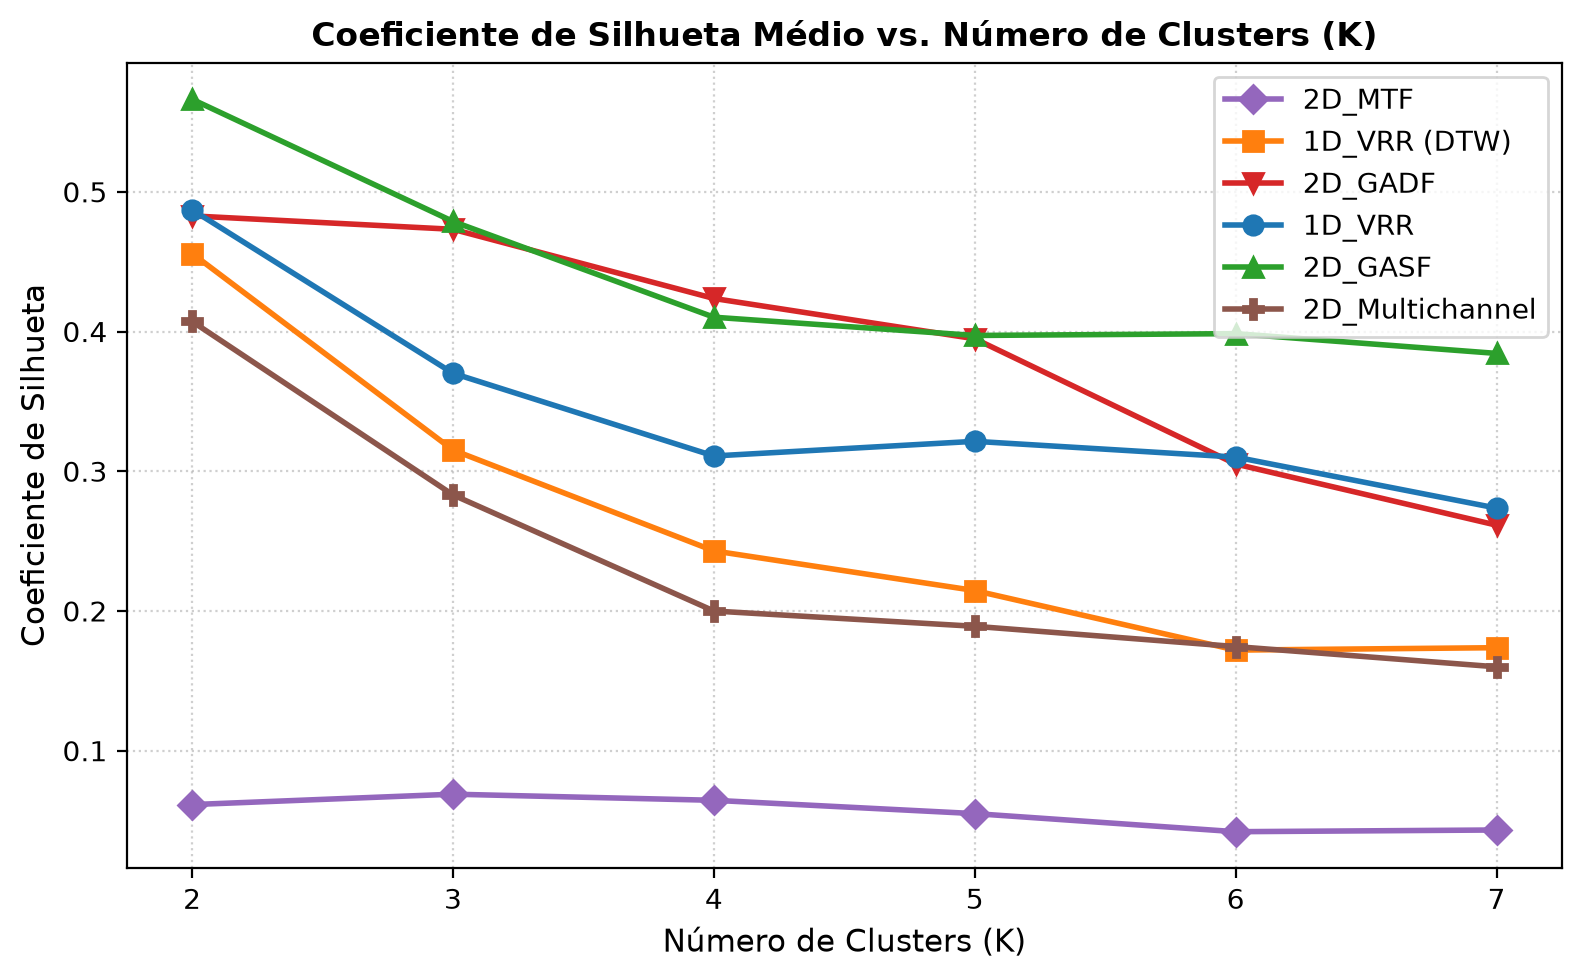
\includegraphics[width=0.85\columnwidth]{../../output/clustering/silhouette_comparison.png}
    \caption{Coeficiente de Silhueta médio para $K \in [2, 7]$ entre representações 1D e 2D.}
    \label{fig:sil_comp}
\end{figure}

\begin{figure}[htbp]
    \centering
    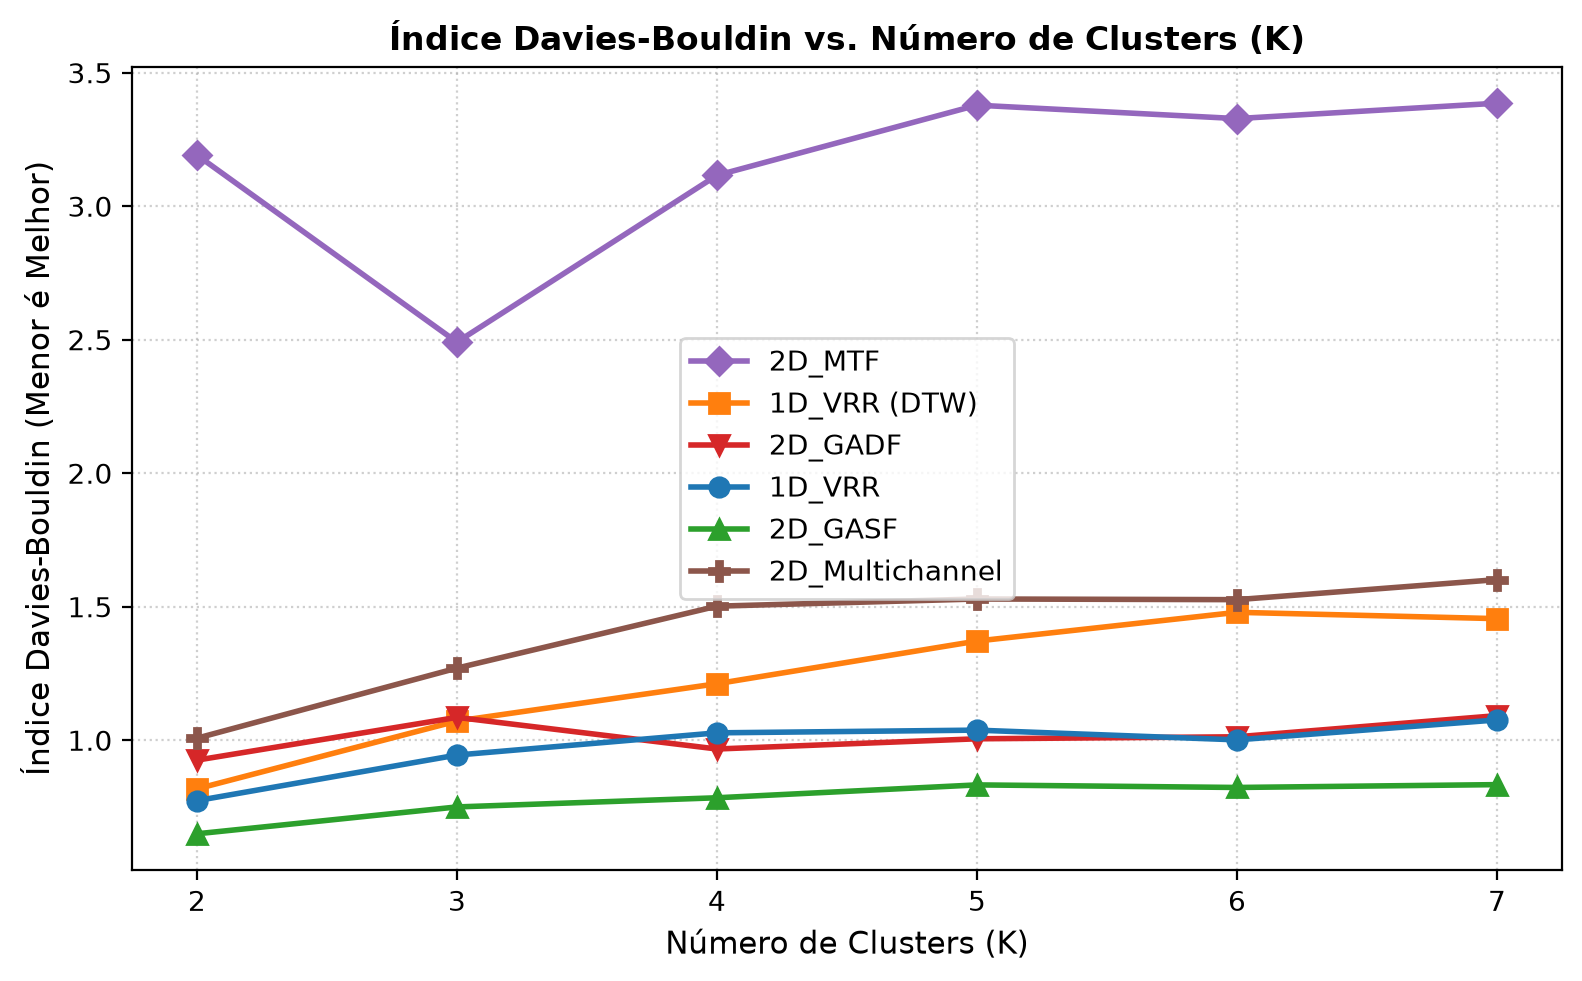
\includegraphics[width=0.85\columnwidth]{../../output/clustering/davies_bouldin_comparison.png}
    \caption{Índice Davies-Bouldin (menor é melhor) para $K \in [2, 7]$.}
    \label{fig:db_comp}
\end{figure}

\begin{figure}[htbp]
    \centering
    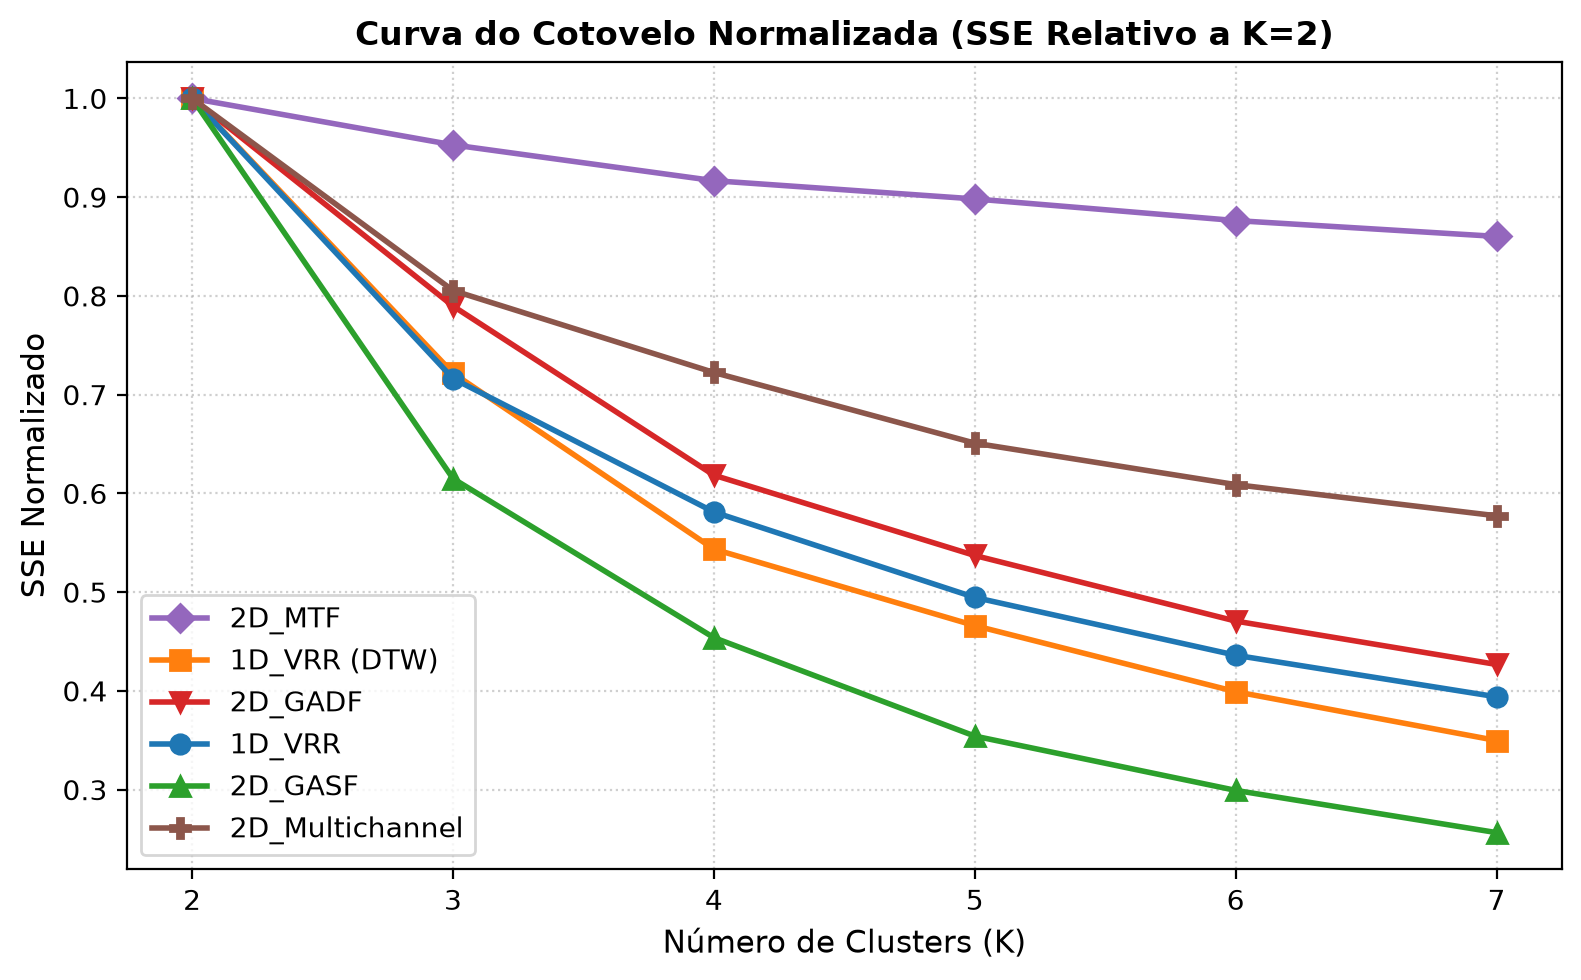
\includegraphics[width=0.85\columnwidth]{../../output/clustering/elbow_normalized_comparison.png}
    \caption{Curvas de decaimento do SSE normalizado em relação a $K=2$ (Método do Cotovelo).}
    \label{fig:elbow_comp}
\end{figure}

\subsubsection{Análise Comparativa 1D vs. 2D}

Os resultados experimentais revelam nuances teóricas de alto valor analítico:
\begin{itemize}
    \item \textbf{Superioridade da Codificação GASF:} O espaço latente derivado do GASF superou consistentemente todas as demais representações em todos os valores de $K$. Em $K=4$, o GASF obteve Silhueta de $+0{,}410$ contra $+0{,}311$ da abordagem 1D Euclidiana e $+0{,}243$ do 1D DTW. O índice Davies-Bouldin correspondente foi substancialmente inferior ($0{,}784$ no GASF frente a $1{,}028$ e $1{,}212$ nas abordagens 1D), comprovando que a transformação angular compacta variações redundantes e amplifica a discriminação de níveis e tendências absolutas de depreciação.
    \item \textbf{Limitações do DTW em Dados Homogêneos:} A métrica DTW apresentou escores de silhueta inferiores aos da distância Euclidiana. Isso ocorre porque o DTW ``perdoa'' defasagens de tempo ao comprimir ou distender o eixo temporal para alinhar curvas. No mercado de veículos, porém, o instante exato em que um ativo se valoriza ou desvaloriza carrega significado econômico vital (p. ex., choque de semicondutores em 2021). Ao flexibilizar o alinhamento de fase temporal, o DTW aglutina veículos com perfis temporais intrinsecamente distintos, gerando grupos com dispersão euclidiana ampliada.
    \item \textbf{Comportamento do MTF:} O campo de transição de Markov apresentou coeficiente de silhueta próximo de zero ($s \approx 0{,}06$) e alto Davies-Bouldin ($DB > 3{,}0$). Essa constatação é coerente com a formulação teórica de \cite{wang2015imaging} e os achados empíricos de \cite{wu2023imaging}: como os quantis do MTF são calculados em nível relativo individual de série, a matriz de transição preserva a dinâmica de oscilação local, mas perde completamente a magnitude absoluta do preço inicial e do VRR final.
\end{itemize}

\subsubsection{Calibração e Desempenho do DBSCAN}

A Figura~\ref{fig:k_dist} exibe os gráficos de $k$-distância gerados para $MinPts = 5$. O joelho pronunciado estabeleceu os parâmetros $\varepsilon = 0{,}104$ para o espaço 1D VRR e $\varepsilon = 0{,}111$ para o espaço 2D GASF.

\begin{figure}[htbp]
    \centering
    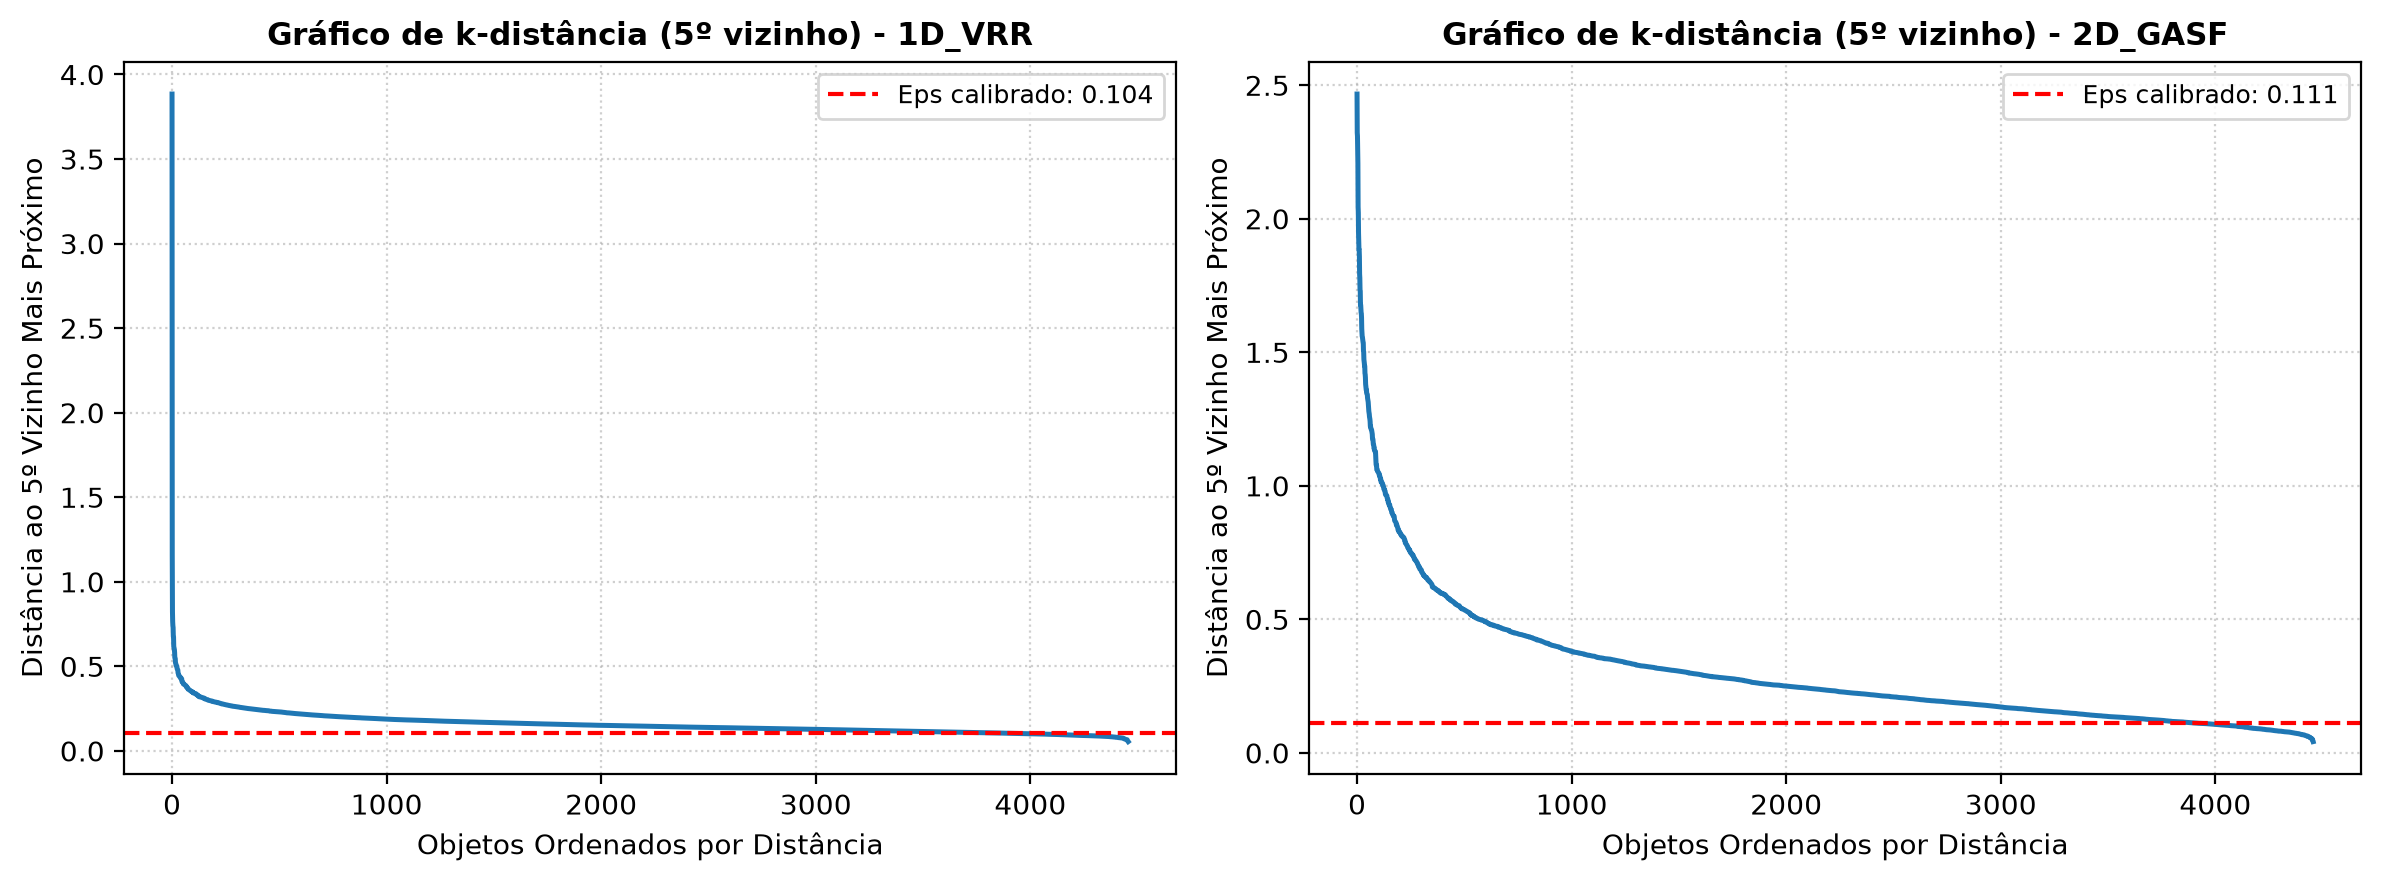
\includegraphics[width=0.9\columnwidth]{../../output/clustering/k_distance_graph.png}
    \caption{Curvas de $k$-distância ordenadas ($MinPts = 5$) e determinação do limiar $\varepsilon$.}
    \label{fig:k_dist}
\end{figure}

O DBSCAN no espaço 1D identificou 39 agrupamentos e classificou $78{,}2\%$ da base como ruído (Silhueta de $-0{,}223$). Já no espaço 2D GASF, o algoritmo particionou instâncias em regiões de alta concentração central (Silhueta dos pontos nucleares de $+0{,}212$). O elevado percentual de ruído evidencia que as trajetórias de depreciação automotiva formam um contínuo com densidade variável e dispersão periférica, justificando a superioridade prática dos métodos particionais (K-Means) para a segmentação de mercado e definição de arquétipos.

\subsection{Caracterização dos Arquétipos de Depreciação \texorpdfstring{($K=4$)}{(K=4)}}

A inspeção da curva do cotovelo (Figura~\ref{fig:elbow_comp}) combinada à interpretabilidade econômica indica que $K=4$ representa o ponto de equilíbrio ótimo para derivar arquétipos comportamentais. A Tabela~\ref{tab:archetypes_summary} sintetiza os quatro perfis identificados pelo modelo 2D GASF, enquanto a Figura~\ref{fig:archetypes_traj} exibe as trajetórias de VRR com seus respectivos intervalos interquartis (Q1--Q3).

\begin{table}[htbp]
\centering
\caption{Síntese dos quatro arquétipos comportamentais de depreciação identificados via 2D GASF ($K=4$).}
\label{tab:archetypes_summary}
\resizebox{\columnwidth}{!}{%
\begin{tabular}{@{} l r r r r r r r r @{}}
\toprule
\textbf{Arquétipo} & \textbf{Veículos} & \textbf{\% Total} & \textbf{VRR 0m} & \textbf{VRR 12m} & \textbf{VRR 32m} & \textbf{$\Delta$ Líquido} & \textbf{Elétricos} & \textbf{\% Eletrif.} \\
\midrule
\textbf{Cluster 1 (Valorização Moderada)}  & 1.005 & 22,5\% & 99,7\% & 116,6\% & 123,0\% & $+23,3\%$ &  14 &  7,5\% \\
\textbf{Cluster 2 (Depreciação Acelerada)} & 1.624 & 36,4\% & 98,6\% & 95,7\%  & 85,0\%  & $-13,6\%$ & 125 & 19,1\% \\
\textbf{Cluster 3 (Super-Valorização)}      &   338 &  7,6\% & 99,9\% & 134,2\% & 139,4\% & $+39,6\%$ &   0 &  3,0\% \\
\textbf{Cluster 4 (Estabilidade Paritária)}& 1.490 & 33,4\% & 99,3\% & 106,1\% & 105,0\% &  $+5,7\%$ &  51 & 11,9\% \\
\bottomrule
\end{tabular}%
}
\end{table}

\begin{figure*}[htbp]
    \centering
    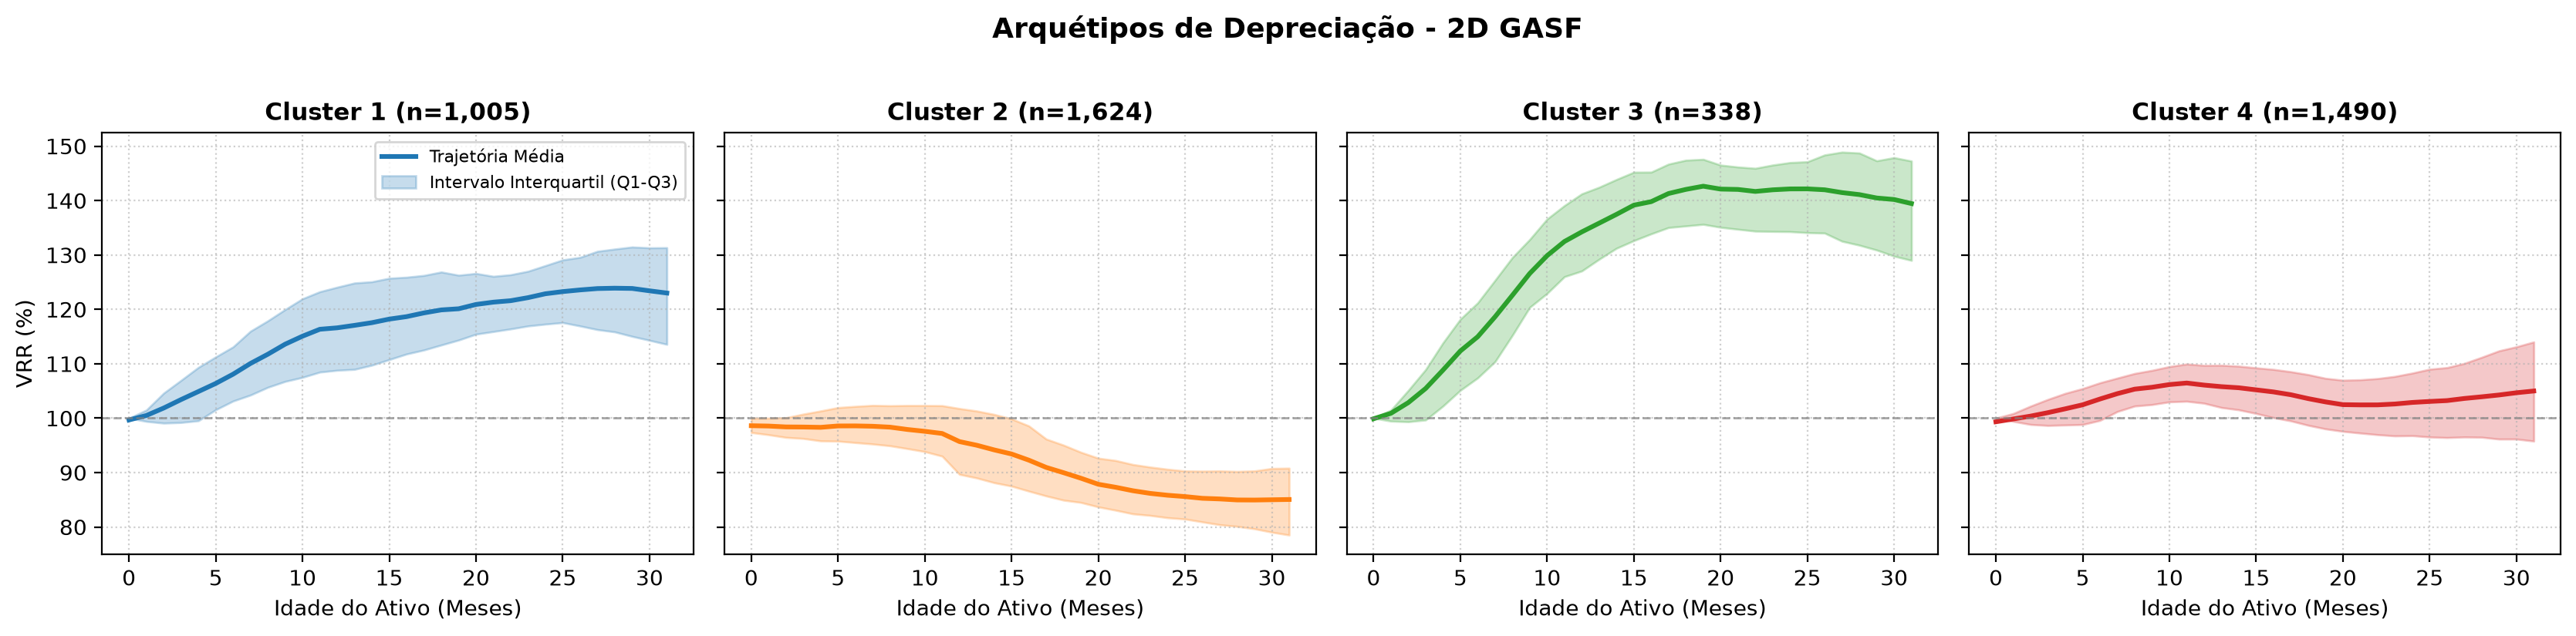
\includegraphics[width=\textwidth]{../../output/clustering/archetypes_trajectories_2d_gasf.png}
    \caption{Trajetórias médias e dispersão interquartil (Q1--Q3) dos quatro arquétipos via 2D GASF.}
    \label{fig:archetypes_traj}
\end{figure*}

Os quatro arquétipos apresentam características operacionais e econômicas nítidas:
\begin{enumerate}
    \item \textbf{Cluster 2 --- Depreciação Acelerada e Perda de Valor:} Reúne 1.624 veículos ($36{,}4\%$ da amostra). Apresenta perda contínua de cotação desde a estreia, fechando aos 32 meses com VRR médio de $85{,}0\%$ (queda acumulada de $-13{,}6\%$). Este agrupamento concentra a grande maioria dos veículos elétricos da base: \textbf{125 de um total de 190 elétricos ($65{,}8\%$ de toda a frota EV)} encontram-se alocados neste cluster, juntamente com 185 modelos híbridos.
    \item \textbf{Cluster 3 --- Super-Valorização Anômala / Utilitários:} Composto por 338 veículos ($7{,}6\%$). Atinge VRR médio de $134{,}2\%$ aos 12 meses e finaliza aos 32 meses em expressivos $139{,}4\%$ de retenção (ganho líquido de $+39{,}6\%$). De forma contundente, \textbf{não há nenhum veículo elétrico neste cluster} ($0$ elétricos e apenas 10 híbridos). O agrupamento é dominado em mais de $97\%$ por veículos a combustão tradicional e utilitários comerciais a diesel, refletindo a explosão de demanda e a escassez de suprimentos no período pandêmico.
    \item \textbf{Cluster 1 --- Valorização Moderada / Resiliência Pós-Pandemia:} Agrupa 1.005 modelos ($22{,}5\%$) com valorização média de $+23{,}3\%$ (VRR final de $123{,}0\%$). Possui representação irrisória de modelos eletrificados ($14$ elétricos, representando apenas $1{,}4\%$ do grupo).
    \item \textbf{Cluster 4 --- Estabilidade e Retenção Paritária:} Reúne 1.490 veículos ($33{,}4\%$) com trajetória resiliente e estável, encerrando aos 32 meses em $105{,}0\%$ do preço inicial ($+5{,}7\%$). Exibe composição mista equilibrada, integrando 51 veículos elétricos e 126 híbridos.
\end{enumerate}

A Figura~\ref{fig:comp_gasf} ilustra a estratificação dos quatro clusters segundo matriz energética e faixa de preço de lançamento. Constata-se que o Cluster 2 (Depreciação Acelerada) absorve a maior concentração percentual de veículos das categorias Intermediário e Luxo eletrificados, evidenciando que a depreciação mais severa incide preponderantemente sobre veículos novos equipados com tecnologia puramente elétrica.

\begin{figure}[htbp]
    \centering
    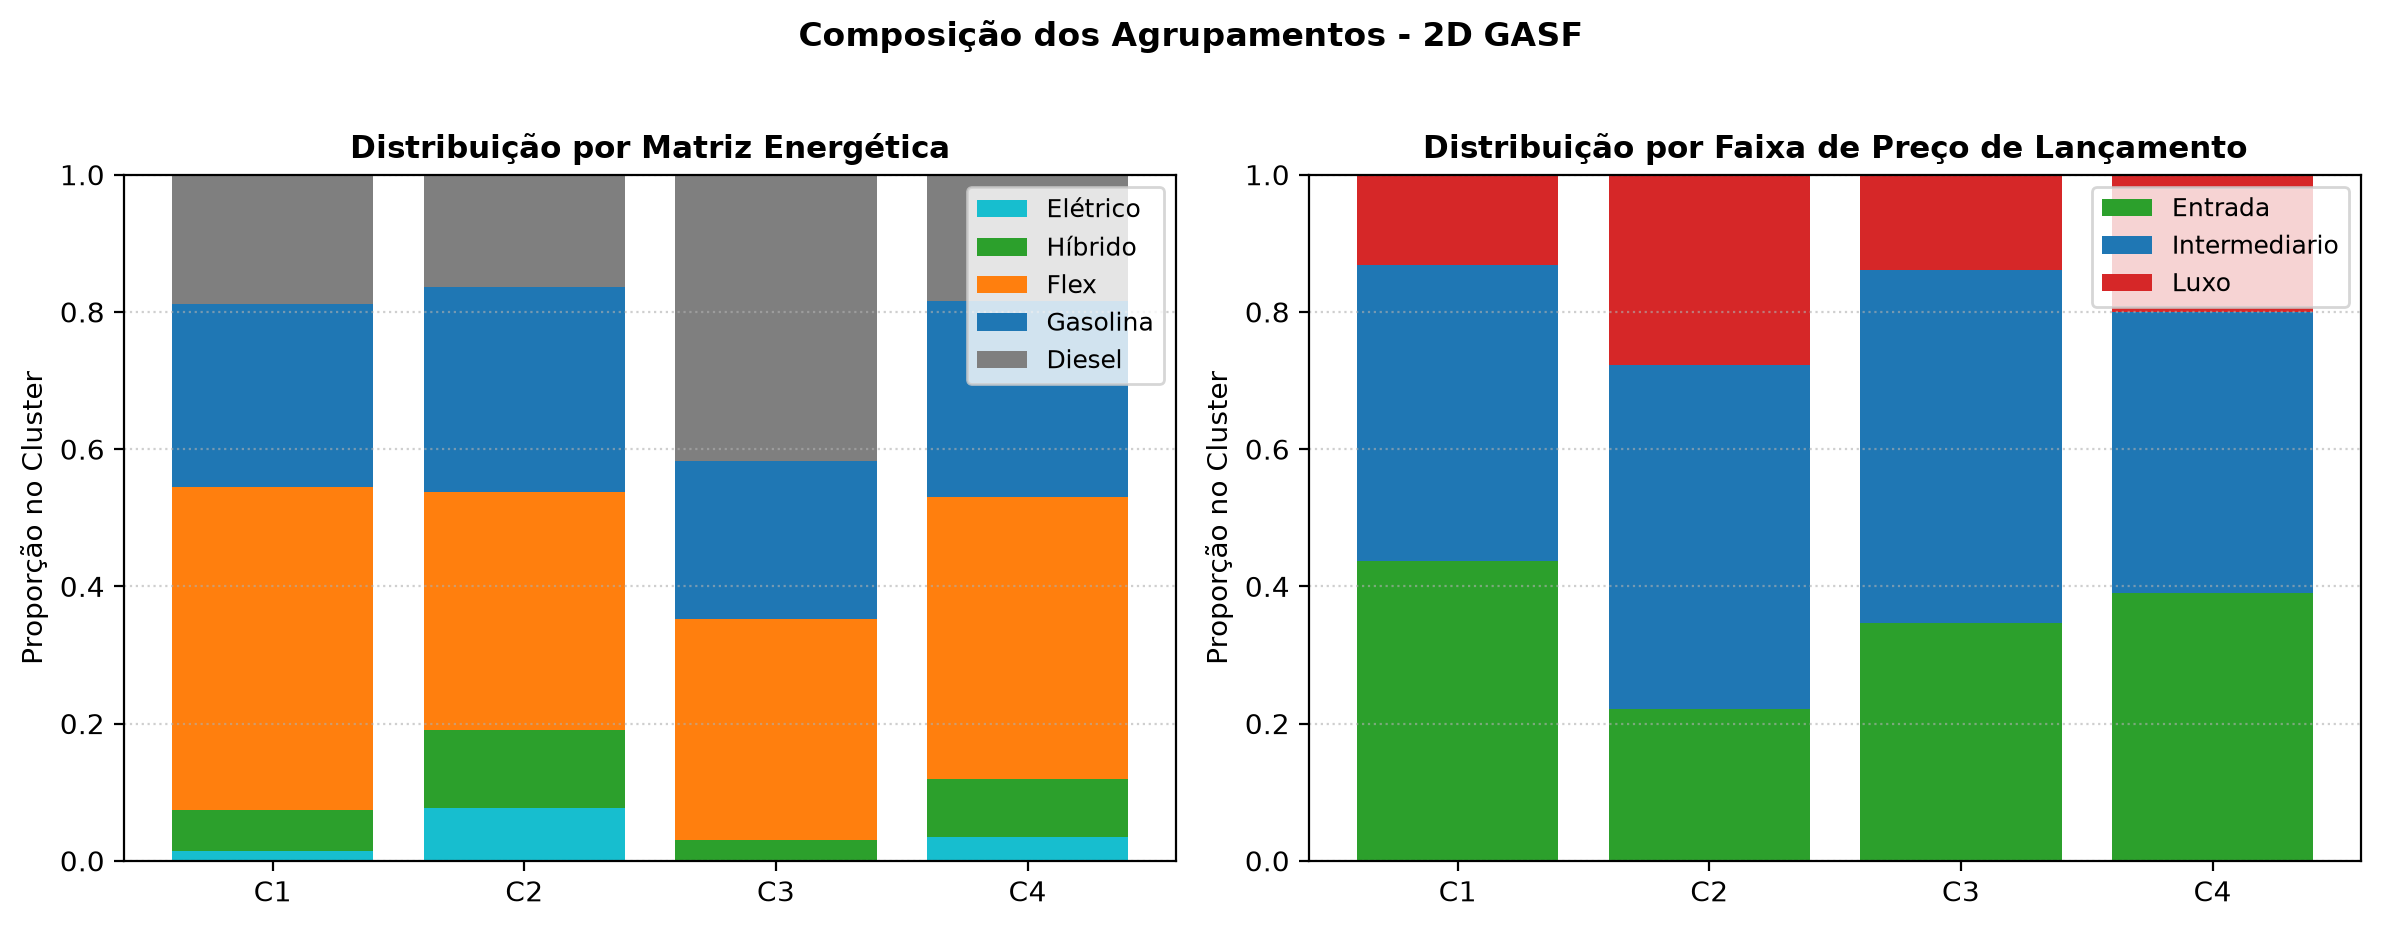
\includegraphics[width=0.9\columnwidth]{../../output/clustering/composition_2d_gasf.png}
    \caption{Composição dos arquétipos segundo tipo de combustível e faixa de preço de lançamento.}
    \label{fig:comp_gasf}
\end{figure}

Por fim, a Figura~\ref{fig:medoids_k4} exibe o medóide representativo de cada um dos quatro arquétipos, conectando a curva temporal de VRR às matrizes correspondentes de GASF, GADF e MTF. O medóide do Cluster 2 (perfil de desvalorização acelerada) exibe contraste angular invertido em relação aos medóides dos clusters em valorização contínua (Clusters 1 e 3), validando visualmente a capacidade das representações espaciais em sintetizar a física de mercado das trajetórias temporais.

\begin{figure*}[htbp]
    \centering
    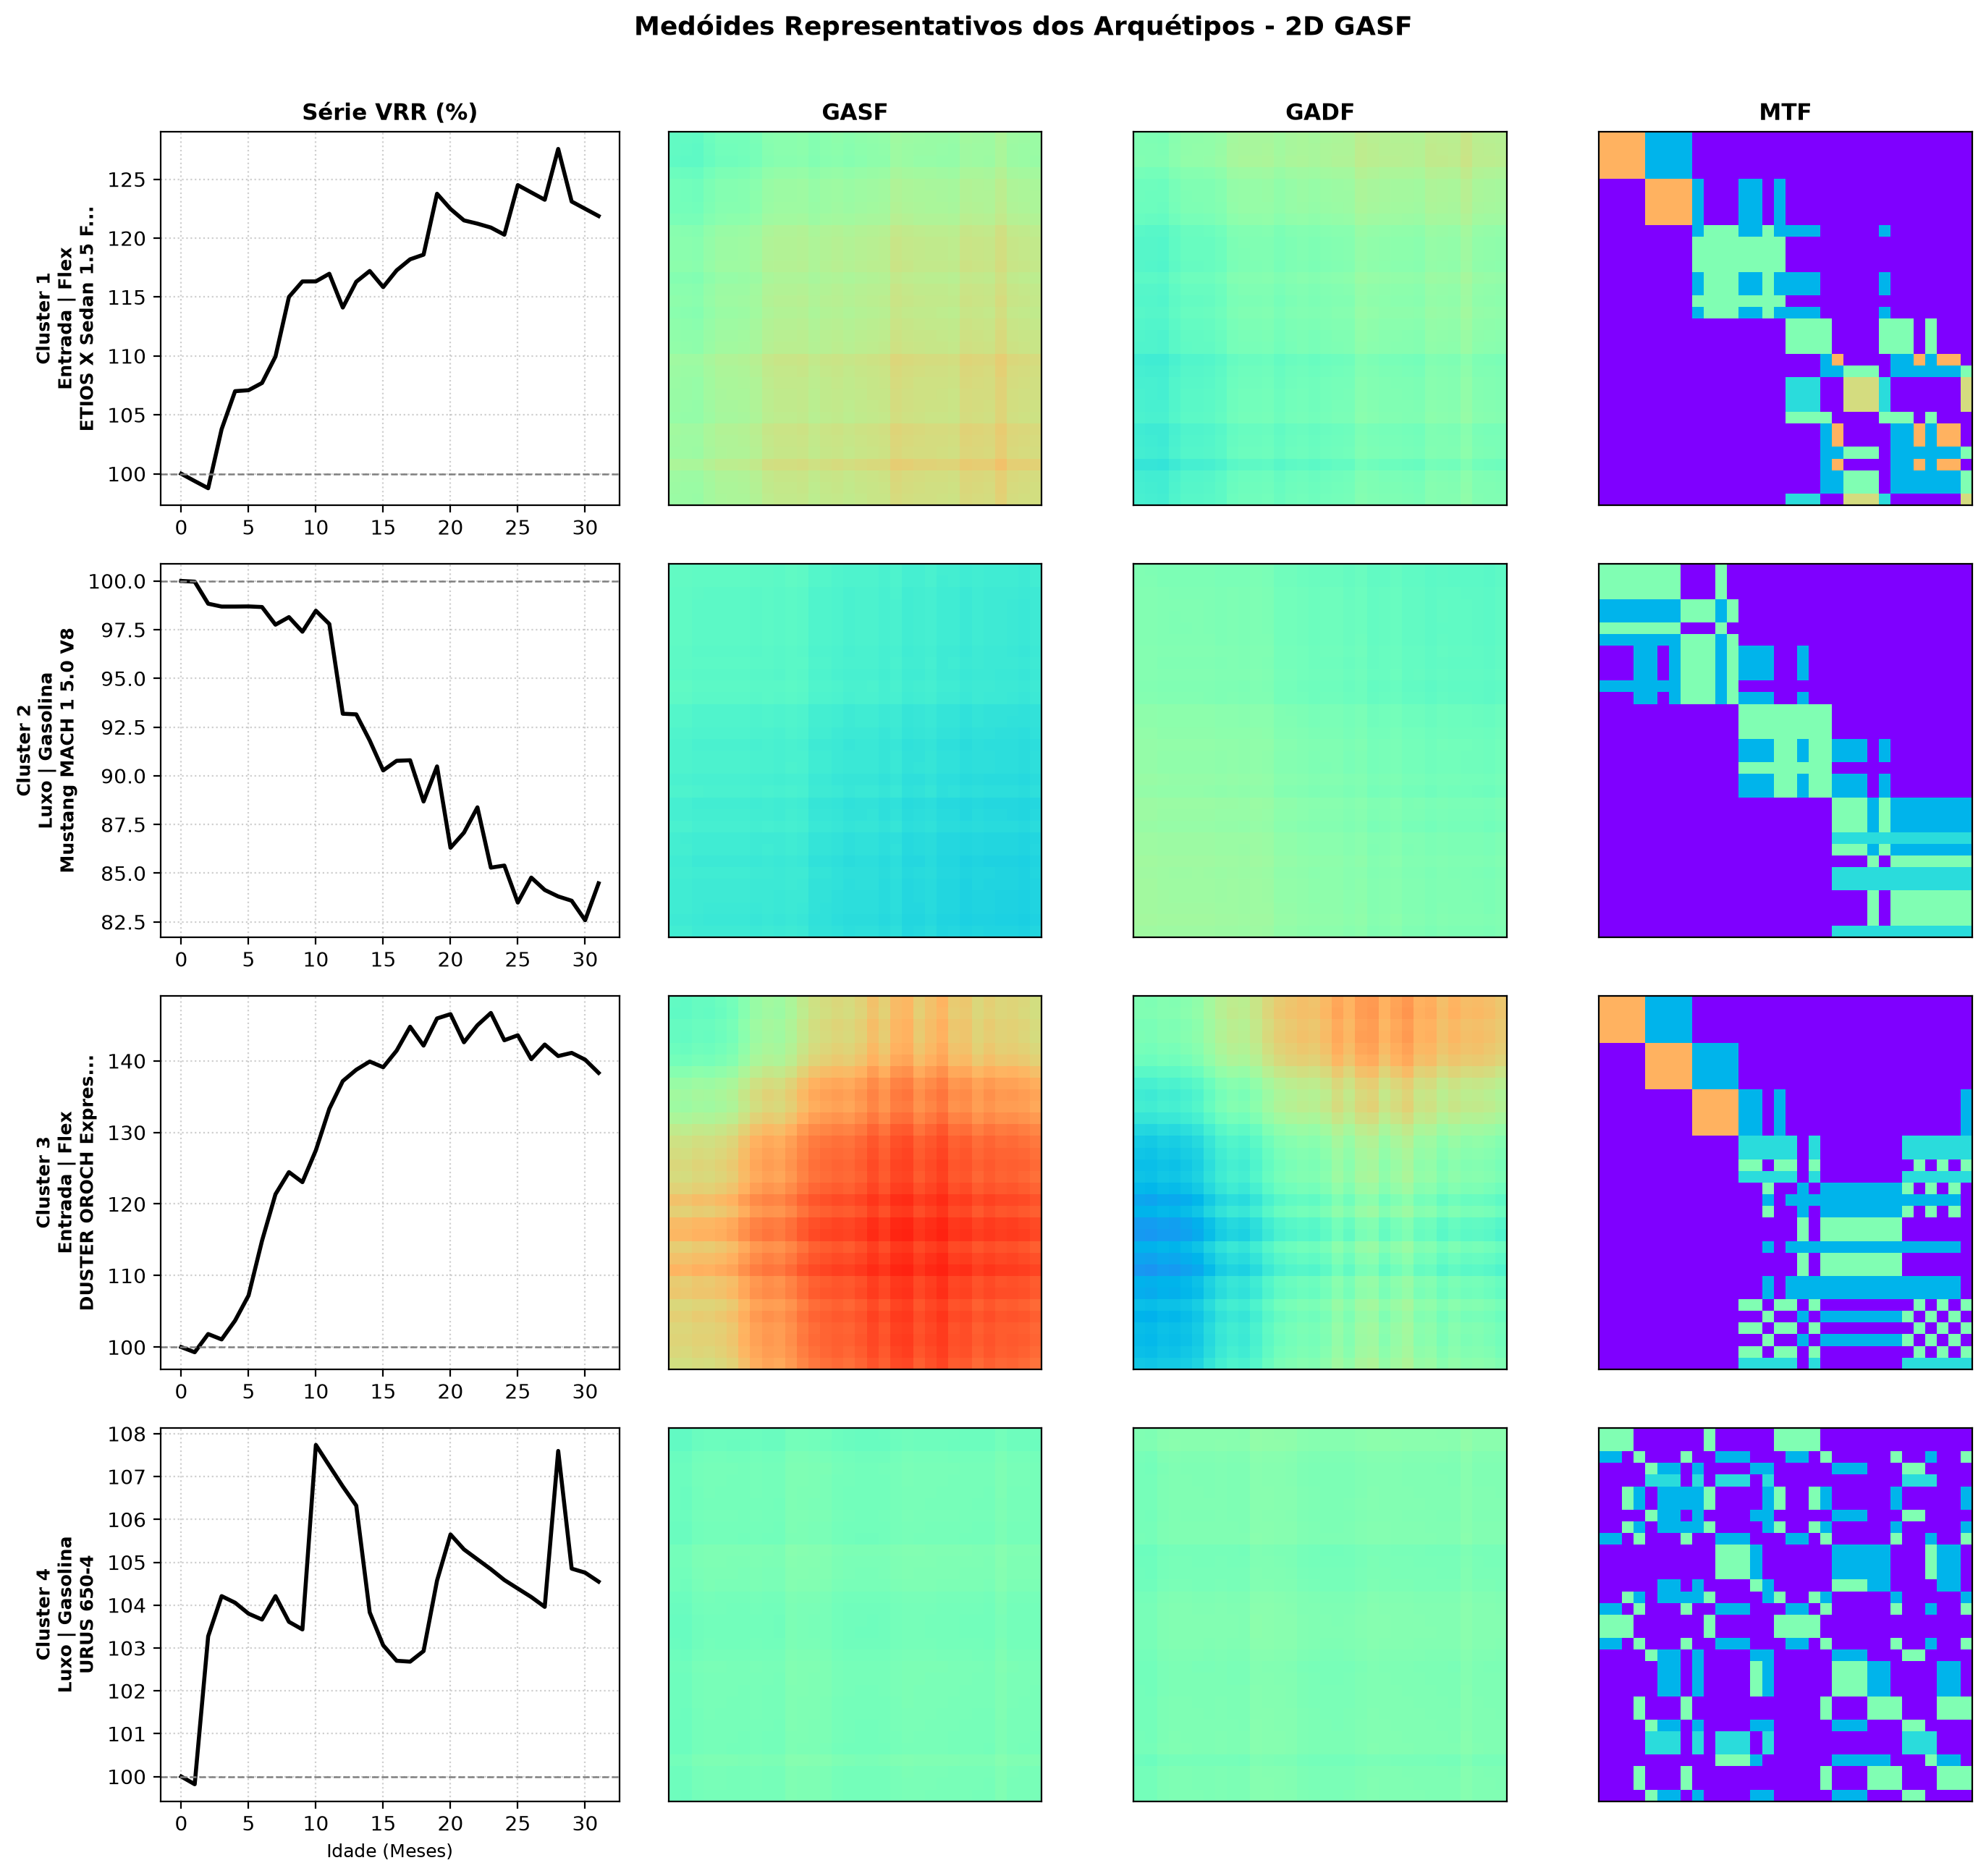
\includegraphics[width=\textwidth]{../../output/clustering/medoids_gasf_k4.png}
    \caption{Medóides representativos de cada arquétipo com suas respectivas séries e imagens 2D (GASF, GADF e MTF).}
    \label{fig:medoids_k4}
\end{figure*}

\subsection{Avaliação Extrínseca: Discriminação de Combustível vs. Faixa de Preço de Lançamento}

Um questionamento metodológico e econômico central na mineração de trajetórias automotivas consiste em verificar se o agrupamento não supervisionado é capaz de identificar e separar os tipos de combustíveis ou se os grupos formados refletem primordialmente as faixas de valores de lançamento dos veículos. Para elucidar essa questão, foram executados testes formais de validação com dados de referência (\textit{ground truth}), decomposição de variância via ANOVA bidirecional e análise de pareamento controlado intra-estrato.

\subsubsection{Métricas Formais de Concordância Extrínseca}

A Tabela~\ref{tab:external_validation} apresenta o cotejamento entre as partições descobertas pelo algoritmo de agrupamento e as duas variáveis de controle externas: o tipo de combustível (5 classes: Flex, Gasolina, Diesel, Híbrido e Elétrico) e o segmento de preço de lançamento (3 classes: Entrada, Intermediário e Luxo).

\begin{table}[htbp]
\centering
\caption{Métricas de validação externa entre os agrupamentos ($K=4$) e as variáveis de controle.}
\label{tab:external_validation}
\small
\resizebox{\columnwidth}{!}{%
\begin{tabular}{@{} l ccccc @{}}
\toprule
\textbf{Variável de Controle} & \textbf{ARI} & \textbf{NMI} & \textbf{Homogeneidade} & \textbf{Completude} & \textbf{V de Cramér} \\
\midrule
Tipo de Combustível           & 0,0117       & 0,0217       & 0,0213                 & 0,0222              & 0,1395               \\
Segmento de Preço             & 0,0121       & 0,0239       & 0,0270                 & 0,0214              & 0,1594               \\
\bottomrule
\end{tabular}%
}
\end{table}

A inspeção dos coeficientes revela que tanto o $\mathrm{ARI} \approx 0{,}012$ quanto o $\mathrm{NMI} \approx 0{,}022$ são muito próximos de zero em relação a ambas as variáveis. Sob a ótica de mineração de dados, esse resultado demonstra que:
\begin{enumerate}
    \item O algoritmo de agrupamento \textbf{não reproduz diretamente nem a etiqueta de combustível nem a faixa de preço nominal}. Como as séries temporais foram normalizadas na origem pela métrica de retenção de valor ($VRR_t = P_t / P_0$), a magnitude nominal em Reais foi descolada da função de distância, de modo que os clusters descrevem estritamente a dinâmica de desvalorização e volatilidade temporal do mercado.
    \item Os escores de concordância frente à faixa de preço e ao tipo de combustível são equivalentes em magnitude, o que refuta a hipótese ingênua de que o agrupamento seja primariamente direcionado pelas faixas de valor do bem.
\end{enumerate}

\subsubsection{Decomposição da Variância: ANOVA Bidirecional}

Para isolar a magnitude com que cada fator governa a variação líquida do valor retido ($\Delta VRR = VRR_{32m} - VRR_{0m}$), formulou-se um modelo de Análise de Variância (ANOVA) bidirecional:
\begin{equation}
\Delta VRR_{i} = \mu + \alpha_{\text{combustivel}, i} + \beta_{\text{preco}, i} + \varepsilon_i.
\end{equation}
Os resultados estatísticos estão consolidados na Tabela~\ref{tab:anova_fuel_price}.

\begin{table}[htbp]
\centering
\caption{ANOVA bidirecional da variação de retenção de valor ($\Delta VRR$) aos 32 meses.}
\label{tab:anova_fuel_price}
\small
\resizebox{\columnwidth}{!}{%
\begin{tabular}{@{} l r c r c @{}}
\toprule
\textbf{Fator Explicativo} & \textbf{Soma dos Quadrados ($SS$)} & \textbf{Graus de Liberdade ($df$)} & \textbf{Estatística $F$} & \textbf{Valor-$p$} \\
\midrule
Tipo de Combustível        & $142.703{,}9$                     & $4$                                & $89{,}51$               & $2{,}80 \times 10^{-73}$ \\
Segmento de Preço          & $73.614{,}5$                      & $2$                                & $92{,}34$               & $5{,}08 \times 10^{-40}$ \\
Resíduos                   & $1.773.727{,}0$                   & $4450$                             & ---                     & ---                      \\
\bottomrule
\end{tabular}%
}
\end{table}

A decomposição da variância evidencia que o \textbf{Tipo de Combustível explica quase o dobro da dispersão das trajetórias de depreciação ($SS = 142.703{,}9$) em relação à Faixa de Preço ($SS = 73.614{,}5$)}, com significância estatística extrema ($p < 10^{-72}$). Portanto, embora o agrupamento não seja uma partição supervisionada de combustíveis, a matriz energética é o principal vetor condutor subjacente à perda ou retenção de valor veicular.

\subsubsection{Concentração de Veículos Elétricos e Análise Controlada Intra-Faixa}

A Figura~\ref{fig:fuel_vs_price_diag} detalha o diagnóstico integrado de concentração e comportamento temporal cruzado.

\begin{figure*}[htbp]
    \centering
    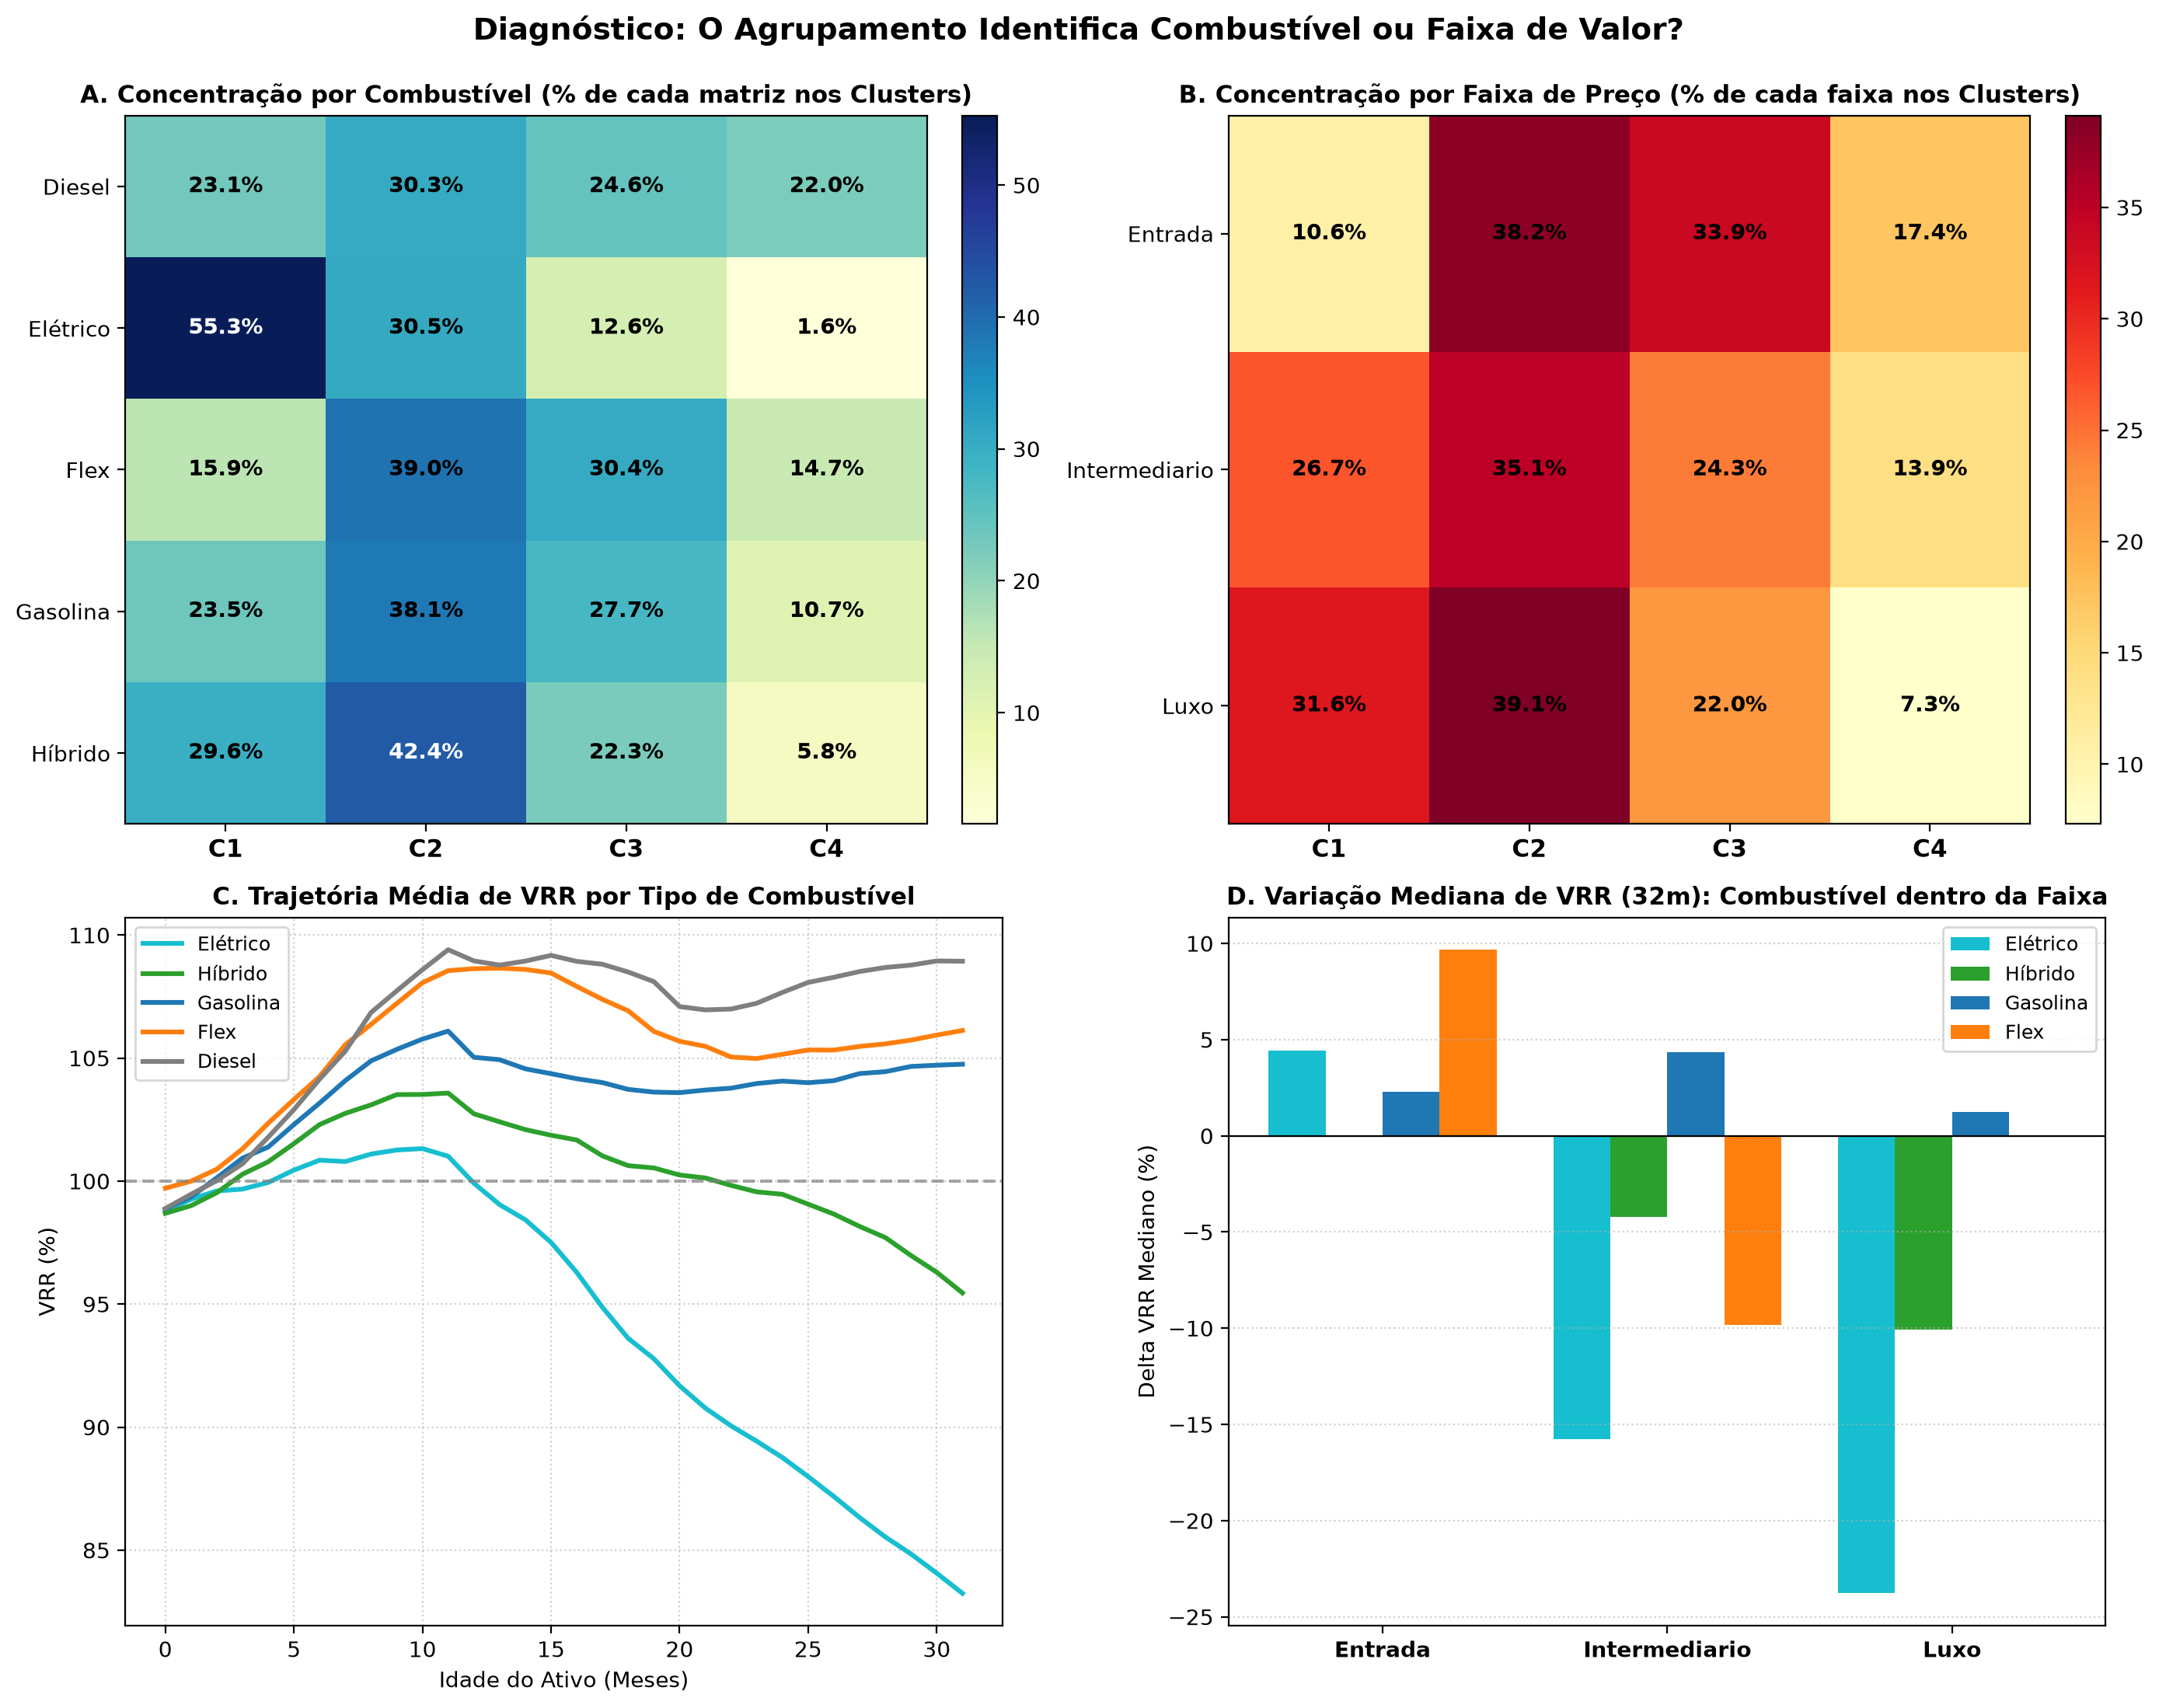
\includegraphics[width=\textwidth]{../../output/clustering/clustering_fuel_vs_price_diagnostic.png}
    \caption{Diagnóstico integrado da influência do tipo de combustível versus faixa de preço de lançamento sobre os agrupamentos. (A) Matriz de concentração percentual de cada matriz energética nos clusters; (B) Matriz de concentração por faixa de preço; (C) Trajetórias médias de VRR por combustível ao longo dos 32 meses; (D) Variação líquida mediana ($\Delta VRR$) controlada por combustível dentro de cada segmento de preço.}
    \label{fig:fuel_vs_price_diag}
\end{figure*}

Os dados ilustrados no painel revelam fenômenos de alto impacto analítico:
\begin{itemize}
    \item \textbf{Concentração Seletiva de Veículos Elétricos (Painel A):} Embora a frota EV represente apenas $4{,}26\%$ do conjunto de dados (190 de 4.457 modelos), mais de metade de toda a amostra elétrica (\textbf{$55{,}26\%$} no espaço 1D e \textbf{$65{,}8\%$} no espaço 2D GASF) é compulsoriamente canalizada para o arquétipo de Depreciação Acelerada (Cluster C1/C2). Em contrapartida, no arquétipo de Super-Valorização (C4/Cluster 3), a presença de elétricos é nula ou residual ($1{,}58\%$, correspondendo a apenas 3 veículos em 190).
    \item \textbf{Controle Intra-Estrato (Painel D):} Ao comparar modelos pareados dentro de uma mesma faixa de preço de lançamento, a divergência entre matrizes energéticas permanece acentuada. No estrato de \textbf{Luxo}, os veículos elétricos sofrem uma perda mediana de $-23{,}78\%$ (média de $-20{,}00\%$) aos 32 meses, ao passo que veículos a gasolina valorizam $+1{,}23\%$ (média de $+5{,}44\%$) e híbridos registram $-10{,}08\%$. Trata-se de uma diferença líquida de mais de \textbf{$25$ pontos percentuais} no mesmo segmento econômico de mercado.
    \item \textbf{Viés de Confundimento e Colinearidade:} A percepção intuitiva de que a depreciação estaria ancorada nas faixas de valor decorre de uma forte assimetria estrutural de mercado: $93{,}2\%$ dos veículos elétricos (177 de 190) custavam acima de R\$ 150 mil na época de lançamento (segmentos Intermediário e Luxo, com preço mediano de R\$ 322 mil), sendo virtualmente inexistentes na faixa de Entrada (apenas 13 veículos). Em contraposição, $75{,}5\%$ dos veículos Flex residem no segmento de Entrada (mediana de R\$ 77 mil). Assim, não é o patamar elevado de preço que causa a desvalorização acelerada, mas sim a concentração de ativos puramente elétricos e híbridos nos estratos superiores de preço, cuja curva de retenção é afetada por obsolescência tecnológica acelerada, degradação de baterias e volatilidade tarifária.
\end{itemize}

